\documentclass{scrartcl}
\usepackage{german}
\usepackage[utf8]{inputenc}
\usepackage[german]{babel}

% zusätzliche mathematische Symbole, AMS=American Mathematical Society
\usepackage{amssymb}
\usepackage{amsmath}
% fürs Einbinden von Graphiken
\usepackage{graphicx}
\usepackage{verbatim}

% für Namen etc. in Kopf- oder Fußzeile
\usepackage{fancyhdr}

% erlaubt benutzerdefinierte Kopfzeilen
\pagestyle{fancy}

% Definition der Kopfzeile
\lhead{
\begin{tabular}{lllll}
Nils Hagner & 4346038 & Felix Karg & 4342014 \\
Michael Fleig & 4340085 & Anush Davtyan &4368689
\end{tabular}
}
\chead{}
\rhead{\today{}}
\lfoot{}
\cfoot{Seite \thepage}
\rfoot{}

\begin{document}

\section*{Solutions for Excercise sheet 3}

\subsection*{Exercise 1 – Requirements Elicitation}
\begin{itemize}
    \item[i] Explicitly different situations represented in the following questions. \\
    \item[ii]
        \verbatiminput{questions.txt}
        Before, those interpretations seemed all plausible:
        \verbatiminput{interpretations.txt}
\end{itemize}



\subsection*{Exercise 2 – Analysis of Decision Tables}

\begin{itemize}
    \item[i]
    \item[ii]
    \item[iii]
    \item[iv]
\end{itemize}

\subsection*{Exercise 3 – Creation of Decision Tables}

\begin{itemize}
    \item[i]
    \item[ii]
    \item[iii]
\end{itemize}
\subsection*{Exercise 4 – Use Cases}

\begin{itemize}
    \item[i]
        \begin{tabular}{|l|l|}
            \hline
            name            & Chack Balance \\ \hline
            goal            & Show specific information about the latest transactions \\ \hline
            pre-condition   & User Authenticated, showing Main Menu, ATM is operational \\ \hline
            post-condition  & showing Main Menu, Maybe printed Summary \\ \hline
            post-condition  & withholding/returning card \\
            in exception-case & and return to authentication screen \\ \hline
            actors          & client (main actor), bank system, printer\\ \hline
            open questions  & none \\ \hline
            normal case     & 1. User Presses 'Balance'-Button \\
                            & 2. get balance-information from bank-system \\
                            & 3. ATM shows Balance-Summary screen \\
                            & 4. User presses confirm \\
                            & 5. returns to Main screen \\ \hline
            normal case 2   & 1. User Presses 'Balance'-Button \\
                            & 2. get balance-information from bank-system \\
                            & 3. ATM shows balance-summary screen \\
                            & 4. User presses print-button \\
                            & 5. disable print-button \\
                            & 6. balance summary will be printed \\
                            & 7. Success-Message appears on screen \\
                            & 8. User pushes confirm button \\
                            & 9. returns to Main screen \\ \hline
            exc. case 0a    & User not responding for 30sec \\
                            & 0.1 withhold card \\
                            & 0.2 return to authentication screen \\ \hline
            exc. case 0b    & Weird sensory data \\
                            & 0b.1 withhold card \\
                            & 0b.2 return to authentication screen \\ \hline
            exc. case 2a    & No connection to bank system could be established \\
                            & 2a.1 show error message \\
                            & 2a.2 show Authentication screen \\
                            & 2a.3 return card \\ \hline
            exc. case 6a    & Printer cannot print \\
                            & 6a.1 Message about not workign printer appears on screen \\
                            & 6a.2 (continue with default point 8) \\ \hline

        \end{tabular}
    \item[ii]
    	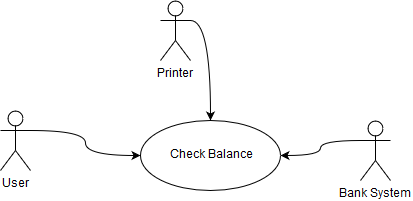
\includegraphics[width=8cm]{use_case_diagram.png} \\
        This use-case diagram only contains the use-case names and the actors.
\end{itemize}

\end{document}
